% options:
% thesis=B bachelor's thesis
% thesis=M master's thesis
% czech thesis in Czech language
% slovak thesis in Slovak language
% english thesis in English language
% hidelinks remove colour boxes around hyperlinks

\documentclass[thesis=M,czech]{FITthesis}[2012/06/26]

\usepackage[utf8]{inputenc} % LaTeX source encoded as UTF-8

\usepackage{graphicx} %graphics files inclusion
% \usepackage[•]{•}kage{amsmath} %advanced maths
% \usepackage{amssymb} %additional math symbols

\usepackage{dirtree} %directory tree visualisation

% % list of acronyms
% \usepackage[acronym,nonumberlist,toc,numberedsection=autolabel]{glossaries}
% \iflanguage{czech}{\renewcommand*{\acronymname}{Seznam pou{\v z}it{\' y}ch zkratek}}{}
% \makeglossaries

\newcommand{\tg}{\mathop{\mathrm{tg}}} %cesky tangens
\newcommand{\cotg}{\mathop{\mathrm{cotg}}} %cesky cotangens

% % % % % % % % % % % % % % % % % % % % % % % % % % % % % % 
% ODTUD DAL VSE ZMENTE
% % % % % % % % % % % % % % % % % % % % % % % % % % % % % % 


\department{Katedra \ldots Počítačové systémy a sítě}
\title{Simulátor akciové burzy}
\authorGN{Jan} %(křestní) jméno (jména) autora
\authorFN{Jůna} %příjmení autora
\authorWithDegrees{Bc. Jan Jůna} %jméno autora včetně současných akademických titulů
\supervisor{Mgr. Jan Starý}
%\acknowledgements{Děkuji své rodině za podporu, svému vedoucímu práce za názory, rady a pomoc a všem ostatním za}
\acknowledgements{Doplňte, máte-li komu a za co děkovat. V~opačném případě úplně odstraňte tento příkaz.}
\abstractCS{Práce se zabývá tvorbou burzovního systému od základních kamenů jako je order matching algoritmus pro spárování burzovních příkazů až po klientské rozhraní umožňující nakupovat nebo prodávat akcie. Aplikace je také tvořena pomocí moderních technologií, jako je Node.JS, Angular.JS, noSQL databáze MongoDB a mnoho dalších. Vše je tvořeno jednodušše a co nejvíce transparentně.}
\abstractEN{Sem doplňte ekvivalent abstraktu Vaší práce v~angličtině.}
\placeForDeclarationOfAuthenticity{V~Praze}
\declarationOfAuthenticityOption{4} %volba Prohlášení (číslo 1-6)
\keywordsCS{akciová burza, realtime aplikace, node.js, angular.js, mongodb, socket.io}
\keywordsEN{stock market, realtime application, node.js, angular.js, mongodb, socket.io}


\begin{document}

% \newacronym{CVUT}{{\v C}VUT}{{\v C}esk{\' e} vysok{\' e} u{\v c}en{\' i} technick{\' e} v Praze}
% \newacronym{FIT}{FIT}{Fakulta informa{\v c}n{\' i}ch technologi{\' i}}

\begin{introduction}
	%sem napište úvod Vaší práce

%\section{Kickoff}

	
\end{introduction}

% ==========================================================================
% ==========================================================================
% ==========================================================================
\chapter{Cíl práce}

V této práci si kladu za cíl prozkoumat a otestovat pro mě nové a zajímavé technologie, naučit se vytvářet single page aplikace, pochopit základní principy burzovních systémů a jeden takový pak také implementovat. Aplikace, kterou budu tvořit a zde také popisovat bude sice pouze jen základní a velmi ořezanou verzí takové opravdové burzy, bude však základním a především i funkčním stavebním kamenem, který se může dále rozvýjet a vylepšovat až do stavu současných burzovních systémů, případně ještě dál. Krom pocitu z nové burzovního systému a získaných vědomostí na poli nových technologií však získám také referenci v a zajímavou poznámku do životopisu.

Mých cílů je tedy doopravdy mnoho, 3 hlavní z nich si ted dúkladněji popíšeme.


\section{Burza}
\section{Nové technologie}
\section{Testování výkonu}

% ==========================================================================
% ==========================================================================
% ==========================================================================
\chapter{Analýza a návrh}

\section{Požadavky}
\section{Koncept systému}
Jak už bylo řečeno výše, celý systém je rozdělen do několika samostatných celků, které spolu komunikují přes síť. Koncept jednotlivých částí si teď zde popíšeme podrobněji.


\subsection{Klientská aplikace}
Klientem se rozumí webová aplikace, která slouží koncovým uživatelům k nakupování a prodávání jejich akcií. Zobrazují se zde aktuální informace o dění na burze a detaily jednotlivých obchodovatelných společností. Klient si tak může zobrazit vývoj ceny akcie a pak podle svého uvážení nakoupit nové nebo prodat jím vlastněné akcie. Kromě aktuálního stavu akcií zde uživatel má také možnost vidět své nakoupené akcie, podané a zatím nevyřízené příkazy a samozřejmě historii všech proběhlých akcí týkajících se uživatele.
Další funkcí je zde registrace, kde se po zadání základních uživatelských údajů vytvoří účet pro obchodování. Při vytváření účtu se uživateli také na účet připíše základní virtuální finanční obnos, za který bude teprve moci nakupovat akcie. V opravdovém systému by toto bylo realizováno ještě nějakou formou platební brány, přes kterou by si klient nabil peníze z reálného účtu. Protože je tato práce zaměřená především na obchodování, v implementaci se zaměříme spíše na základní a klíčové části burzy, jako je samotné obchodování.
    Po úspěšné registraci uživatele máme možnost příhlásit se. Tato funkce se jako jediná provádí na straně serveru, kde se data z přihlašovacího formuláře nejprve odešlou na REST API umístěnou u brokera. Ten přihlašovací údaje ověří, odešle zpět výsledek přihlašování. V případě neúspěšného přihlášení klient obdrží chybovou hlášku, v opačném případě pak klíč, který bude dále používat při volání dotazů na REST API brokera. Při přihlášení si klientská aplikace tento klíč uloží do session a odešle uživateli do prohlížeče aplikaci napsanou v javascriptovém frameworku angular.js. Tato aplikace si pak sama obsluhuje routování (přechod mezi stránkami), zobrazování jednotlivých pohledů (view v MVC frameworku), zpracování a načítání dat z externích zdrojů.
    Jednou z dalších možností, jak udělat uživatelské přihlášení je odesílat přihlašovací údaje rovnou z uživatelského prohlížeče na API brokera. Důvodem, proč v mé práci data nejprve odesílám na server klientské aplikace a až poté odtud kontaktuji brokera je, že vlastní aplikaci na obchodování posílám klientovi až při úspěšném přihlášení. Pro nepřihlášené uživatele je zobrazena pouze stránka s přihlášením a registrací. Nepřihlášení uživatelé tak nemohou získat potenciálně citlivé informace, jako jsou například volané adresy na REST API u brokera, bez toho, aniž by se nejprve přihlásili. 
    V klientské aplikaci také pro ukládání sessions použivám key-value databázi Redis, která v případě více spuštěných nodů poslouží jako společné úložiště sjednocující všechny sessions do jednoho místa. Více o výhodách použití Redis databáze si řekneme v sekci škálování.
    Při přihlášení klient začne komunikovat s REST API brokera, přes kterou si načítá veškerá data o uživateli. Protože může býkace s REST APt klientská aplikace umístěna na jiné doméně, než broker, probíhá komuniI pomocí CORS (Cross-origin resource sharing) mechanismu. To není nic jiného, než posílání ajax requestů na externí adresu, která však musí ve svých hlavičkách tento mechanismus povolit. Více k této metodě využívání externích zdrojů si uvedeme v popisu aplikace brokera. Přes tento komunikační kanál pak probíhá také zadávání BUY a SELL pokynů. Kromě RESTu zde používám také Socket.IO, což je nástroj pro obousměrnou komunikaci klienta i serveru. V praxi tak může server posílat push notifikace (zprávy o změně stavu) bez předchozího klientského dotazu (donedávna se toto řešilo cyklickým dotazováním klienta na nový stav, kdy velká zátěž byla tvořena neustálým a často i zbytečnými klientskými dotazy. Takto si server s clientem udržuje stálé spojení a až v případě změny stavu server sám upozorní klienta. V klientské aplikaci je tato technologie použita například při načítání nových provedených příkazů. Veškerá komunikace by se dala předělat jen na použití Socket.IO nebo opačně jen na REST, ale protože si v této práci kladu za cíl i naučit se nové technologie, využil jsem obě možnosti podle vhodnosti každé z nich.
    Pro vizuální stránku jsem použil free a open source šablonu AdminLTE, která svým přehledným rozhraním a responzivním chováním poskytuje uživateli přijemný pocit z používání aplikace.


\subsubsection{Robot}
\subsubsection{Propojení s brokerem}

\subsection{Broker}
\subsubsection{Robot}

\subsection{Burza}
\subsubsection{Jádro}
\subsubsection{Rozhraní}

\subsection{Komunikace mezi celky}

\section{Použité technologie}

\subsection{Angular.js}

\includegraphics[width=0.8\textwidth]{images/logo_angularjs}

Počátek vývoje této technologie sahá pouze do roku 2010, jde tedy o relativně novou technologii, která však již dnes přináší mnoho nástrojů a funkcí pro jednoduchý a především rychlý vývoj SPA (single page application) aplikací. Základní vlastností je, že se zobrazení výsledné stránky a jednoduché transformace dat provádí u klienta. To umožňuje odlehčit komunikaci na přenos pouze základní aplikace, která si poté už dotahuje pouze potřebná data. Ta pak na jednotlivých částech aplikace postupně zobrazuje. Kromě snížení přenášených dat zde dochází také k výraznému odlehčení zátěže na serveru, kdy se většina výpočtů deleguje na klienta. Tím se operace prováděné na serveru zredukují pouze na nejzákladnější práci s databází a podobně. Prostředí pro klientské výpočty, renderování vzhledu a mnoho dalšího zajištujě právě open source MVC (model-view-controller) framework angular.js běžící v prohlížeči na straně klienta. Pomocí tohoto nástroje můžeme nadefinovat zobrazení jednotlivých stránek (view) a k nim pak controllery, které tyto zobrazení obsluhují. Controllery se dotazují nejčastěji přes nějakou formu API (v našem případě REST api realizované pomocí Node.JS) na data (model) a ty poté předávají do view, kde se teprve vykreslují a prezentují uživateli. Most mezi view a controllerem zajišťuje komponenta nazvaná “scope”, která zajišťuje obousměrné předávání dat mezi těmito dvěma vrstvami. Tato vlastnost je v terminologii angularu nazvaná two way data binding a je jednou z klíčových vlastností v tomto frameworku. Při změně dat v controlleru (například při dotažení nových dat z REST API) dojde totiž k automatickému promítnutí i do view vrstvy a naopak, při změně dat ve view (například úpravě položky ve formuláři) se data ihned promítnou i v controlleru.
Svou jednoduchostí a schopností raketově urychlit vývoj výsledné aplikace si angular.js oblíbila spousta webových vývojářu. Jeho použití však není omezeno pouze na webové aplikace. S příchodem technologií jako je Phonegap nebo Titanium se dá nasadit také na mobilních zařízeních a tabletech. Phonegap zde slouží jako prostředník mezi mobilní API a aplikací napsanou v technologiích HTML5 a JavaScript, což může být právě aplikace napsaná v angularu. Nejedná se pak sice o nativní aplikaci a takové použití rozhodně není určeno pro náročné aplikace jako jsou například hry a nebo nástroje provádějící složité výpočetní operace. Technologie jako je například již zmíněný Phonegap však sjednocuj API mnoha mobilních zařízeních a systémů a jedna aplikace napsaná v HTML a JavaScriptu se tak může použít na všech takto podporovaných zařízeních. Nejen to, ale také možňost vytvořit jednu společnou aplikaci pro mobily a pro web výrazně urychlí vývoj a sníží náklady na hromadu programátorů, kteří by jinak tvořili samostatné nativní aplikace na každé požadované prostředí. Angular.JS se tedy používá také jako první otestování bussines plánu, kdy se rychle vytvoří prvotní verze aplikace a až podle úspěchu a uživatelského zájmu se začne pracovat na nativních aplikacích.
Z těchto a mnoha dalších důvodů jsem se rohodl v mé práci použít právě angular.JS. Spolu s dalšími technologiemi tvoří právě již zmíněný MEAN stack, což je čtveřice v současnosti hojně používaných technologií pro tvorbu startup aplikací.


\subsection{Nginx}


\includegraphics[width=0.8\textwidth]{images/logo_nginx}

Nginx je další z použitých open source technologií, jejíž jedno možné použití je nasazení jako web server zajišťující vysoký výkon. V naší práci jej však použijeme jako Load balancer, který bude sloužit jako prostředník mezi uživatelem a backendem realizovaným pomocí node.js. Nejedná se o jediný možný použitelný Load balancer, je však jeden z nejznámějších, a proto ho použijeme i v našem případě.
V základní verzi naší aplikace bude sloužit pouze jako proxy čekající na HTTP spojení na portu 80. Traffic jdoucí na tento port bude přesměrovávat na konkrétní zadaný port používaný naší aplikací. V reálném nasazení se nginx používá také pro load balancing, kdy se backend aplikací spustí více, popřípad se v aplikacích použije ještě clustering, kdy se se node.js aplikace rozprostře na více jader a těchto aplikací se spustí více na více počítačích a pomocí load balancingu se pak rozhazují jednotlivé požadavky mezi tyto nody. To nám zajistí vysoký výkon naší aplikace a především také vysokou horizontální škálovatelnost, kdy pro zvýšení výkonu nám stačí pouze přidat další server a zapojit ho do load balancingu. O možnostech škálování si budeme více povídat v kapitole Škálování.

\subsection{Node.JS}


\includegraphics[width=0.8\textwidth]{images/logo_nodejs}


Node.JS je jednou z klíčových technologií v této práci, jedná se o nástroj umožňující stavět multiplatformní škálovatelné aplikace běžící na systému Windows, Mac OS X i Linux. Jádro zde představuje V8 JavaScript engine vytvořený společností Google, který byl použit mimo jiné i v prohlížeči Chrome pro zpracování JavaScriptu. V roce 2009 byl tento interpretr vzat a spolu s pár dalšími knihovnami nasazen na serveru, čímž se vytvořilo prostředí pro spuštění javascriptového kódu jako server-side aplikace. Kromě V8 enginu se node skládá z knihoven, které jsou napsány buď v jazyce C a C++ a nebo přímo v JavaScriptu.
Psaní programů v Node.JS je téměř srovnatelná s tvorbou JavaScript aplikací v prohlížeči. Rozdílem je zde, že byla odebrána podpora pro práci s DOM modely. Přidáno pak bylo rozhraní pro práci se síťovou komunikací a především také funkcionalita na snadné vytvoření TCP/IP nebo přímo HTTP serveru.
Jednou ze základních principů nejenom nodu, ale i celého javascriptu je orientace na eventy (event driven programming), kdy se spíše než používání návratových hodnot z funkcí pomocí klíčového slova return používají callback funkce. Vše můžeme uvést na příkladu se čtením ze souboru, kdy místo toho, abychom zkoumali návratovou hodnotu z čtecí funkce, pošleme spolu s příkazem na čtení také speciální funkci (callback funkce), která se zavolá až dojde k načtení dat. Pomocí vlastnosti neblokujících i/o operací (nonblocking i/o) se v nodu zpracování nezastaví a nečeká se na načtení dat. Místo toho se pokračuje dál a zatím se provádí další operace. Při načtení dat se teprve zavolá callback funkce, která teprve data obslouží. Právě I/O operace zabírají nejvíce času a node.js svým neblokujícím zpracováním toto zbytečné čekání odstranil. Tyto vlastnosti a fakt, že je z velké části psán v jazyce C/C++ mu dávají ohromnou rychlost a výkonnostní náskok před jeho ekvivalenty.
Mezi velké přednosti Nodu patří i jeho modulárnost, kdy se celá aplikace rozděluje do modulů, které se až poté spojují do funkčního celku. Těchto modulů je na světě ohromné množství, z nichž téměř 70 tisíc bylo uvolněno samotnými uživateli také pro veřejnost. Pokud pak někdo tvoří aplikaci například s uživatelským přihlášením, může se nejprve podívat, zda již někdo nevytvořil modul, který by tuto funkčnost zajištoval. Pro snadné hledání a indexaci vytvořených modulů vznikla také stránka www.npmjs.org, která umožňuje rychlé hledání ve veřejných modulech.
    
    
\subsection{Express.JS}


\includegraphics[width=0.8\textwidth]{images/logo_express}


\subsection{Redis}


\includegraphics[width=0.8\textwidth]{images/logo_redis}

Redis je jedna z klíčových složek škálovatelnosti Node.JS aplikací. Jejím hlavním cílem je sloužit jako malá a jednoduchá, ale zároveň i velmi rychlá databáze slučující data z více serverů. Do této databáze se tak nejčastěji ukládají “cache”, které server použává, aby odlehčil a zmírnil přílišné dotazování se do databáze. Jako dalším častým příkladem dat ukládaných do Redisu jsou uživatelské sessions, což řeší problém, kdy se například při rozhazování zátěže pomocí load balancingu přepošlou data s uživatelskou registrací na jeden server, zde dojde k přihlášení, ale na druhém serveru již uživatel není znám. Pokud by pak load balancer přesměroval uživatelův požadavek na jiný server, z důvodu absence session by byl pak považován za nepřihlášeného a jeho požadavek by mohl být zamítnut. Takto mají všechny aplikační servery společné úložiště, které zajištujě, že pokud se uživatel přihlásí na jednom serveru, bude přihlášen i na všech ostatních.


\subsection{MongoDB}


\includegraphics[width=0.8\textwidth]{images/logo_mongodb}

\subsection{Socket.IO}


\includegraphics[width=0.8\textwidth]{images/logo_socketio}

\section{Bezpečnost}
\section{Škálovatelnost}


% ==========================================================================
% ==========================================================================
% ==========================================================================
\chapter{Realizace}

\section{Klient}
\section{Broker}
\subsection{Broker robot}
\section{Burza}
\subsection{OrderMatching}

% ==========================================================================
% ==========================================================================
% ==========================================================================
\chapter{Testování}

\section{Testování kódu}
\subsection{Nastavení unit testů}
\subsection{Unit testy}

\section{Zátěžové testy}
\subsection{Testované prostředí}
na jakém stroji probíhá testování
\subsection{Testovací scénář}
jaké jsou testovaní scénáře
\subsubsection{Scénář 1 - rychlost odezvy}
text a grafy
\subsubsection{Scénář 1 - rychlost odezvy}
text a grafy
\subsubsection{Scénář 1 - rychlost odezvy}
text a grafy
\subsubsection{Scénář 1 - rychlost odezvy}
text a grafy
\subsubsection{Scénář 1 - rychlost odezvy}
text a grafy
\subsection{Výsledky měření}

\subsection{Závěr měření}

% ==========================================================================
% ==========================================================================
% ==========================================================================
\chapter{Deployment}

\section{Správa kódu}
\section{Nasazení na serveru}
\subsection{Instalace závislostí}
\subsection{Stažení zdrojového kódu}
\subsection{Nastavení prostředí}
\subsection{Spuštění}

% ==========================================================================
% ==========================================================================
% ==========================================================================
\chapter{Monitoring}

\section{Monitorování serveru}
\section{Debugging běžícího serveru}

% ==========================================================================
% ==========================================================================
% ==========================================================================
\chapter{Škálování}



\begin{conclusion}

Práce žádný závěr nemá...

\end{conclusion}

\bibliographystyle{csn690}
\bibliography{mybibliographyfile}

\appendix

\chapter{Seznam použitých zkratek}
% \printglossaries
\begin{description}
	\item[GUI] Graphical user interface
	\item[XML] Extensible markup language
\end{description}


% % % % % % % % % % % % % % % % % % % % % % % % % % % % 
% % Tuto kapitolu z výsledné práce ODSTRAŇTE.
% % % % % % % % % % % % % % % % % % % % % % % % % % % % 
% 
% \chapter{Návod k~použití této šablony}
% 
% Tento dokument slouží jako základ pro napsání závěrečné práce na Fakultě informačních technologií ČVUT v~Praze.
% 
% \section{Výběr základu}
% 
% Vyberte si šablonu podle druhu práce (bakalářská, diplomová), jazyka (čeština, angličtina) a kódování (ASCII, \mbox{UTF-8}, \mbox{ISO-8859-2} neboli latin2 a nebo \mbox{Windows-1250}). 
% 
% V~české variantě naleznete šablony v~souborech pojmenovaných ve formátu práce\_kódování.tex. Typ může být:
% \begin{description}
% 	\item[BP] bakalářská práce,
% 	\item[DP] diplomová (magisterská) práce.
% \end{description}
% Kódování, ve kterém chcete psát, může být:
% \begin{description}
% 	\item[UTF-8] kódování Unicode,
% 	\item[ISO-8859-2] latin2,
% 	\item[Windows-1250] znaková sada 1250 Windows.
% \end{description}
% V~případě nejistoty ohledně kódování doporučujeme následující postup:
% \begin{enumerate}
% 	\item Otevřete šablony pro kódování UTF-8 v~editoru prostého textu, který chcete pro psaní práce použít -- pokud můžete texty s~diakritikou normálně přečíst, použijte tuto šablonu.
% 	\item V~opačném případě postupujte dále podle toho, jaký operační systém používáte:
% 	\begin{itemize}
% 		\item v~případě Windows použijte šablonu pro kódování \mbox{Windows-1250},
% 		\item jinak zkuste použít šablonu pro kódování \mbox{ISO-8859-2}.
% 	\end{itemize}
% \end{enumerate}
% 
% 
% V~anglické variantě jsou šablony pojmenované podle typu práce, možnosti jsou:
% \begin{description}
% 	\item[bachelors] bakalářská práce,
% 	\item[masters] diplomová (magisterská) práce.
% \end{description}
% 
% \section{Použití šablony}
% 
% Šablona je určena pro zpracování systémem \LaTeXe{}. Text je možné psát v~textovém editoru jako prostý text, lze však také využít specializovaný editor pro \LaTeX{}, např. Kile.
% 
% Pro získání tisknutelného výstupu z~takto vytvořeného souboru použijte příkaz \verb|pdflatex|, kterému předáte cestu k~souboru jako parametr. Vhodný editor pro \LaTeX{} toto udělá za Vás. \verb|pdfcslatex| ani \verb|cslatex| \emph{nebudou} s~těmito šablonami fungovat.
% 
% Více informací o~použití systému \LaTeX{} najdete např. v~\cite{wikilatex}.
% 
% \subsection{Typografie}
% 
% Při psaní dodržujte typografické konvence zvoleného jazyka. České \uv{uvozovky} zapisujte použitím příkazu \verb|\uv|, kterému v~parametru předáte text, jenž má být v~uvozovkách. Anglické otevírací uvozovky se v~\LaTeX{}u zadávají jako dva zpětné apostrofy, uzavírací uvozovky jako dva apostrofy. Často chybně uváděný symbol "{} (palce) nemá s~uvozovkami nic společného.
% 
% Dále je třeba zabránit zalomení řádky mezi některými slovy, v~češtině např. za jednopísmennými předložkami a spojkami (vyjma \uv{a}). To docílíte vložením pružné nezalomitelné mezery -- znakem \texttt{\textasciitilde}. V~tomto případě to není třeba dělat ručně, lze použít program \verb|vlna|.
% 
% Více o~typografii viz \cite{kobltypo}.
% 
% \subsection{Obrázky}
% 
% Pro umožnění vkládání obrázků je vhodné použít balíček \verb|graphicx|, samotné vložení se provede příkazem \verb|\includegraphics|. Takto je možné vkládat obrázky ve formátu PDF, PNG a JPEG jestliže používáte pdf\LaTeX{} nebo ve formátu EPS jestliže používáte \LaTeX{}. Doporučujeme preferovat vektorové obrázky před rastrovými (vyjma fotografií).
% 
% \subsubsection{Získání vhodného formátu}
% 
% Pro získání vektorových formátů PDF nebo EPS z~jiných lze použít některý z~vektorových grafických editorů. Pro převod rastrového obrázku na vektorový lze použít rasterizaci, kterou mnohé editory zvládají (např. Inkscape). Pro konverze lze použít též nástroje pro dávkové zpracování běžně dodávané s~\LaTeX{}em, např. \verb|epstopdf|.
% 
% \subsubsection{Plovoucí prostředí}
% 
% Příkazem \verb|\includegraphics| lze obrázky vkládat přímo, doporučujeme však použít plovoucí prostředí, konkrétně \verb|figure|. Například obrázek \ref{fig:float} byl vložen tímto způsobem. Vůbec přitom nevadí, když je obrázek umístěn jinde, než bylo původně zamýšleno -- je tomu tak hlavně kvůli dodržení typografických konvencí. Namísto vynucování konkrétní pozice obrázku doporučujeme používat odkazování z~textu (dvojice příkazů \verb|\label| a \verb|\ref|).
% 
% \begin{figure}\centering
% 	
\includegraphics[width=0.5\textwidth, angle=30]{cvut-logo-bw.pdf}
% 	\caption[Příklad obrázku]{Ukázkový obrázek v~plovoucím prostředí}\label{fig:float}
% \end{figure}
% 
% \subsubsection{Verze obrázků}
% 
% % Gnuplot BW i barevně
% Může se hodit mít více verzí stejného obrázku, např. pro barevný či černobílý tisk a nebo pro prezentaci. S~pomocí některých nástrojů na generování grafiky je to snadné.
% 
% Máte-li například graf vytvořený v programu Gnuplot, můžete jeho černobílou variantu (viz obr. \ref{fig:gnuplot-bw}) vytvořit parametrem \verb|monochrome dashed| příkazu \verb|set term|. Barevnou variantu (viz obr. \ref{fig:gnuplot-col}) vhodnou na prezentace lze vytvořit parametrem \verb|colour solid|.
% 
% \begin{figure}\centering
% 	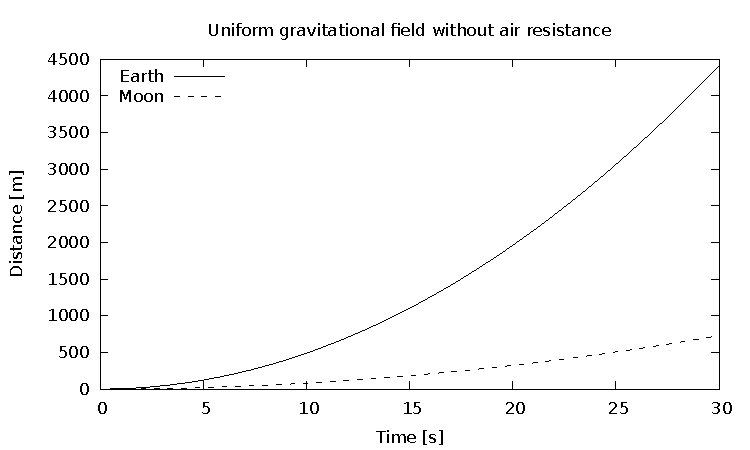
\includegraphics{gnuplot-bw}
% 	\caption{Černobílá varianta obrázku generovaného programem Gnuplot}\label{fig:gnuplot-bw}
% \end{figure}
% 
% \begin{figure}\centering
% 	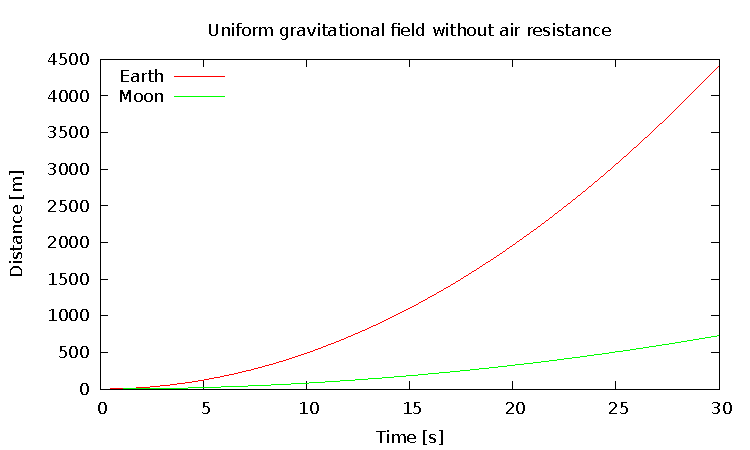
\includegraphics{gnuplot-col}
% 	\caption{Barevná varianta obrázku generovaného programem Gnuplot}\label{fig:gnuplot-col}
% \end{figure}
% 
% 
% \subsection{Tabulky}
% 
% Tabulky lze zadávat různě, např. v~prostředí \verb|tabular|, avšak pro jejich vkládání platí to samé, co pro obrázky -- použijte plovoucí prostředí, v~tomto případě \verb|table|. Například tabulka \ref{tab:matematika} byla vložena tímto způsobem.
% 
% \begin{table}\centering
% 	\caption[Příklad tabulky]{Zadávání matematiky}\label{tab:matematika}
% 	\begin{tabular}{|l|l|c|c|}\hline
% 		Typ		& Prostředí		& \LaTeX{}ovská zkratka	& \TeX{}ovská zkratka	\tabularnewline \hline \hline
% 		Text		& \verb|math|		& \verb|\(...\)|	& \verb|$...$|		\tabularnewline \hline
% 		Displayed	& \verb|displaymath|	& \verb|\[...\]|	& \verb|$$...$$|	\tabularnewline \hline
% 	\end{tabular}
% \end{table}
% 
% % % % % % % % % % % % % % % % % % % % % % % % % % % % 

\chapter{Obsah přiloženého CD}

%upravte podle skutecnosti

\begin{figure}
	\dirtree{%
		.1 readme.txt\DTcomment{stručný popis obsahu CD}.
		.1 exe\DTcomment{adresář se spustitelnou formou implementace}.
		.1 src.
		.2 impl\DTcomment{zdrojové kódy implementace}.
		.2 thesis\DTcomment{zdrojová forma práce ve formátu \LaTeX{}}.
		.1 text\DTcomment{text práce}.
		.2 thesis.pdf\DTcomment{text práce ve formátu PDF}.
		.2 thesis.ps\DTcomment{text práce ve formátu PS}.
	}
\end{figure}

\end{document}
